Connecting fuzzy logic and artificial neural networks one has a lot of choices on the type of system hybrydization (connection).
One can distinguish two main types of fuzzy neural networks: 
\begin{itemize}
\item Cooperative FNNs,
\item Hybrid FNNs.
\end{itemize}

\subsubsection{Cooperative fuzzy neural networks}
Speaking of cooperative neural fuzzy systems, both artificial neural network and fuzzy system work independently from each other.

\begin{wrapfigure}{r}{0.71\textwidth}
	%\captionsetup{width=18pc}
	\vspace*{-1.5em}
	%\hspace*{1.5em}
	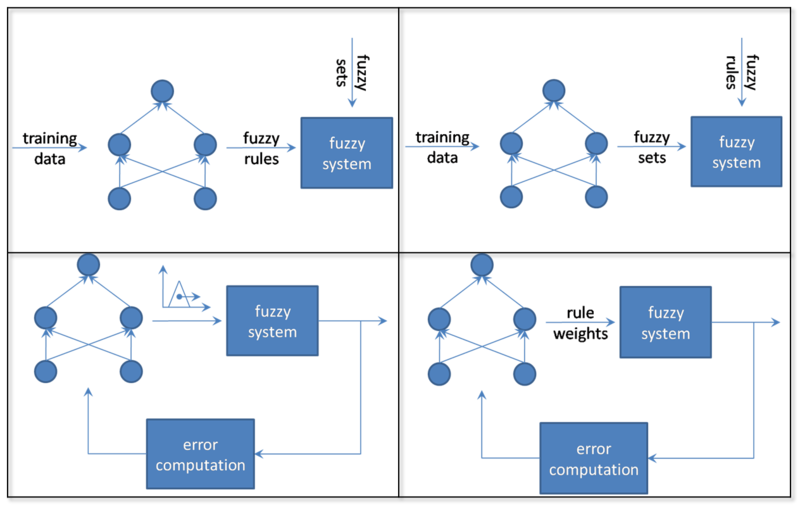
\includegraphics[width=0.72\textwidth]{images/fnn_cooperative_types.png}
	%[height=0.4\textheight,keepaspectratio]
	\caption{Different types of cooperative fuzzy neural networks~\cite{scholarpedia_fuzzy_neural}.}
	\label{fig:fnn_cooperative}
\end{wrapfigure}

The artificial neural network tries to learn the parameters from the fuzzy system. This can be either performed offline or online while the fuzzy system is applied.
Figure~\ref{fig:fnn_cooperative} depicts four different kinds of cooperative fuzzy neural networks.

The upper left fuzzy neural network learns fuzzy set from given training data.
This is usually performed by fitting membership functions with a neural network.
The fuzzy sets are then determined offline.
They are then utilized to form the fuzzy system by fuzzy rules that are given (not learned) as well.

The upper right neuro-fuzzy system determines fuzzy rules from training data by a neural network.
Here as well, the neural networks learns offline before the fuzzy system is initialized.
The rule learning usually done by clustering on self-organizing feature maps.
It is also possible to apply fuzzy clustering methods to obtain rules.

In the lower left neuro-fuzzy model, the system learns all membership function parameters online, i.e., while the fuzzy system is applied. Thus initially fuzzy rules and membership functions must be defined beforehand. Moreover, the error has to be measured in order to improve and guide the learning step.

The lower right one determines rule weights for all fuzzy rules by a neural network. This can be done online and offline. A rule weight is interpreted as the influence of a rule.
They are multiplied with the rule output.
Here the problem is that the semantics of rule weights are not clearly defined.
They could be replaced by modified membership functions.
However, this could destroy the interpretation of fuzzy sets.
Moreover, identical linguistic values might be represented differently in dissimilar rules.

% ====================================================
\subsubsection{Hybrid fuzzy neural networks}

Hybrid neuro-fuzzy systems are homogeneous and usually resemble neural networks.
Here, the fuzzy system is interpreted as special kind of neural network.
The advantage of such hybrid NFS is its architecture since both fuzzy system and neural network do not have to communicate any more with each other.
They are one fully fused entity.
These systems can learn online and offline.
One can see a model of that type of FNN in Figure~\ref{fig:fnn_hybrid}.

\begin{wrapfigure}{r}{0.6\textwidth}
	%\captionsetup{width=18pc}
	\vspace*{-1.5em}
	%\hspace*{1.5em}
	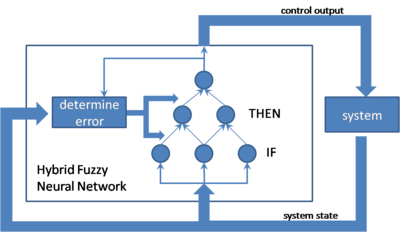
\includegraphics[width=0.6\textwidth]{images/fnn_hybrid.png}
	%[height=0.4\textheight,keepaspectratio]
	\caption{Hybrid fuzzy neural network model~\cite{scholarpedia_fuzzy_neural}.}
	\label{fig:fnn_hybrid}
\end{wrapfigure}

The rule base of a fuzzy system is interpreted as a neural network.
Fuzzy sets can be regarded as weights whereas the input and output variables and the rules are modeled as neurons.
Neurons can be included or deleted in the learning step.
Finally, the neurons of the network represent the fuzzy knowledge base.
Obviously, the major drawbacks of both underlying systems are thus overcome.
In order to build a fuzzy controller (set of rules), membership functions which express the linguistic terms of the inference rules have to be defined.
In fuzzy set theory, there does not exist any formal approach to define these functions.
Any shape (e.g., triangular, Gaussian) can be considered as membership function with an arbitrary set of parameters.
Thus the optimization of these functions in terms of generalizing the data is very important for fuzzy systems.
Neural networks can be used to solve this problem.
By fixing a distinct shape of the membership functions, say triangular, the neural network must optimize their parameters by gradient descent.
Thus, aside information about the shape of the membership functions, training data must be available as well.
Another approach is to group the training data $$ \{(x_i,y_i) | x_i \in X, y_i \in Y, i = 1,2,\dots,l\}$$to $M$ clusters.
Every cluster represents a rule $R_m$ where $m=1,2,\dots,M$.
Hence these rules are not defined linguistically but rather by crisp data points $x=(x_1, x_2, \dots,x_n)$.
Thus a neural network with $n$ input units, hidden layers and $M$ output units might be applied to train on the pre-defined clusters.
For testing, an arbitrary pattern $x$ is presented to the trained neural network.
Every output unit $m$ will return a degree to which extend $x$ may fit to the antecedent of rule $R_m$.

To guarantee the characteristics of a fuzzy system, the learning algorithm must enforce the following mandatory constraints:
\begin{itemize}
\item Fuzzy sets must stay normal and convex,
\item Fuzzy sets must not exchange their relative positions (they must not pass each other),
\item Fuzzy sets must always overlap.
\end{itemize}

Additionally there do exist some optional constraints like the following:
\begin{itemize}
\item Fuzzy sets must stay symmetric,
\item The membership degrees must sum up to 1 (as mentioned in section~\ref{ssec:fuzzy_neurons})
\end{itemize}
